\chapter{Background}
\section{The ARM big.LITTLE Architecture}
The ARM big.LITTLE~\cite{samsung, Greenhalgh2011} is a state-of-the-art AMC architecture that has been successfully deployed in the mobile market. The observation that mobile devices typically combine phases with low and high computational demands motivated this original design. ARM big.LITTLE combines simple in-order cores with aggressive out-of-order cores in the same System-on-Chip (SoC) to provide high performance and low power. \textit{Big} and \textit{little} cores support the same architecture so they can run the same binaries and therefore easily combined within the same system.
%Recent generations of the big.LITTLE processor further improve the system peak performance by allowing to use all the cores in the system simultaneously.
% 
Current cores implementing the ARMv7-A and ARMv8-A ISA support big.LIT\-TLE configurations. 
%Thus, the available cores to act as \textit{little} cores are the ARM Cortex-A7, A35 and A53, while the available \textit{big} cores are the ARM Cortex-A15, A17, A57, A72 and A73.

The little cores in a big.LITTLE system are designed targeting energy efficiency. Current implementations have relatively short pipelines with up to dual-issue in-order execution. L1 caches are split for instructions and data and can be dimensioned according to the target domain from 8 to 64 KB in size~\cite{MPR_A53}. The big cores are designed for high performance. Current designs
have deeper pipelines with up to seven-issue out-of-order execution, increased number of functional units and improved floating-point capabilities. L1 data cache is up to 64 KB and L1 instruction cache is up to 64 KB\cite{MPR_A57, MPR_A72,GWENAPP}. Little and big cores are typically integrated in a hierarchical manner. A set of cores form a cluster that may include a cache that is shared among cores in the cluster~\cite{GWENAPP}. Then, multiple clusters can be interconnected through an on-chip network and share a last-level cache and connection to main memory and peripherals.

\begin{figure}[t]
        \centering
        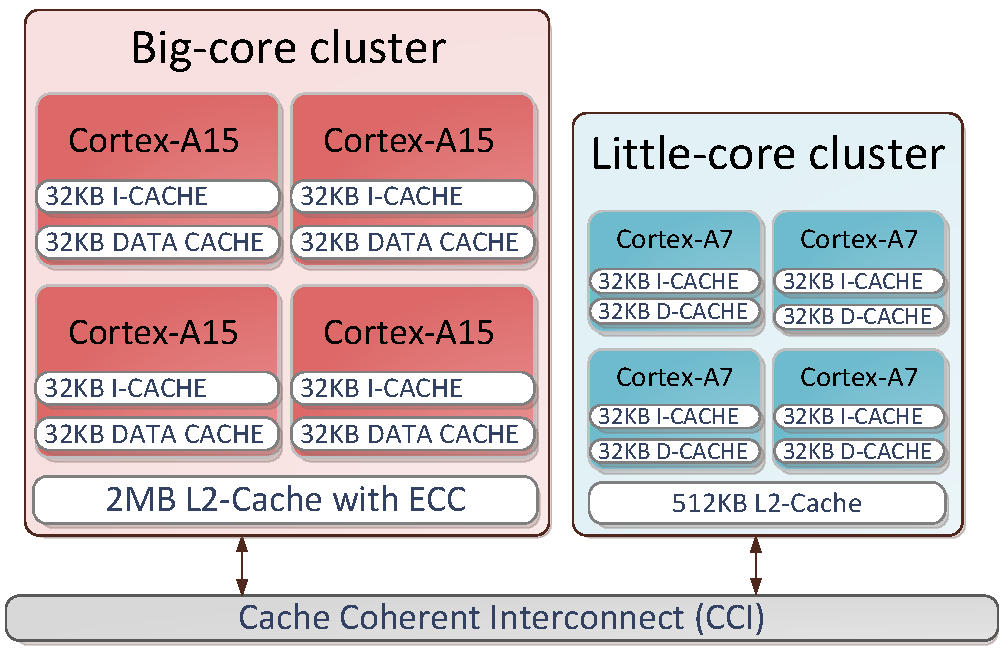
\includegraphics[width=\columnwidth]{figures/block_diagram.pdf}%
        \caption{Samsung Exynos 5422 processor with ARM big.LITTLE architecture.}%
        \label{fig:big-little-diagram}%
        \vspace{-0.56cm}
\end{figure}

In this work, we use of one of the commercially available development boards featuring a big.LITTLE architecture: the Hardkernel Odroid-XU3 development board. As shown in Figure~\ref{fig:big-little-diagram}, the Odroid-XU3 includes an 8-core Samsung Exynos 5422 chip with four ARM Cortex-A15 cores and four Cortex-A7 cores. The four Cortex-A15 share a 2~MB 16-way 64-byte-cache-line L2 cache, while the Cortex-A7 cores share a 512~KB L2 cache. A single memory controller provides access to 2~GB of LPDDR3 RAM with dual 32-bit channels at 1866~MT/s. The reason we use this platform instead of the more up-to-date Juno platform~\cite{Juno} is that even if the latter features the more advanced Cortex~A53 and Cortex~A57 cores, it is limited to six cores instead of the 8 cores in Odroid-XU3.


%Odroid gives us the opportunity to evaluate up to eight cores while Juno, even if it features the more advanced Cortex~A53 and Cortex~A57 cores, is limited to only six total cores. 

The Cortex-A7 cores in this SoC support dual-issue of instructions and their pipeline length is between 8 and 10 stages. The L1 instruction cache is 32KB two-way set associative, with virtually indexed and physically tagged cache-lines that can hold up to 8 instructions. The core supports instruction prefetch by predicting the outcome of branches; the prefetch unit can fetch up to a maximum of four instructions per cycle. The L1 data cache is four-way set associative with physically-indexed and physically-tagged cache lines and uses a pseudo-random replacement policy \cite{TRM_A7}. Dynamic Voltage and Frequency Scaling (DVFS) techniques adjust the frequency of the little cores from 200MHz up to 1.4GHz.

The Cortex-A15 cores in this SoC support triple-issue of instructions and their pipeline length is 
between 15 and 24 stages~\cite{MPR_A15}. The L1 instruction and data caches of the Cortex-A15 are 
both 32~KB and 2-way set-associative with 64~byte cache lines. The processor supports speculative 
instruction execution by maintaining a 2-level global history-based dynamic predictor 
with a branch target buffer~\cite{TRM_A15}. The instruction decode unit performs register renaming 
to remove the Write-After-Write and the Write-After-Read hazards, and promote 
instruction reordering~\cite{TRM_A15}. The instruction dispatch unit analyzes instruction dependences 
before issuing them for execution.  The integer execute unit includes 2 
Arithmetic Logical Units with support for operand forwarding. DVFS techniques vary the 
frequency of the big cores from 200~MHz up to 2~GHz.
For the rest of the paper, we refer to Cortex-A15 cores as \textit{big} and to Cortex-A7 cores as \textit{little}.


%\mm{Explain different pipelines.} \mm{Number of execution units per pipeline?} \mm{ROB size? Maximim number of in-flight instructions?}.  As in the little cores, the data and instruction L1 caches are 32KB each. \mm{FLOPS single and double precision?}.

%In the big.LITTLE processor, the four Cortex-A15 cores form a \emph{cluster} with a shared L2 cache (16-way set-associative with 64 bytes line size), while the Cortex-A7 form a second cluster with a smaller shared L2 cache (8-way 64 bytes cache-line size). This asymmetric multi-core implements the ARMv7 instruction set architecture on all the cores. The two clusters are coherent, so a single shared memory application can run on both clusters, using up to eight cores simultaneously. For the cluster-to-cluster communication, the processor features a cache coherent interconnect. This mechanism allows big and little cores to exchange data at low cost as if they were effectively in the same cluster. Figure~\ref{fig:big-little-diagram} shows a block diagram of such processor.




%%%%%%%%%%%%%%%%%%%
%%%%%%%%%%%%%%%%%%%
% \subsection{Challenges in Scheduling}
% 
% Scheduling a set of processes on an asymmetric multi-core system with big.LITTLE architecture is trickier than the traditional process scheduling on homogeneous multi-cores. 
% An efficient OS scheduler has to take into account the different characteristics of the core types of the system.
% ARM supports two different approaches on scheduling chips with big.LITTLE architecture: the \textit{cluster switching}, and the \textit{global task scheduling}. In this paper we evaluate a different approach which is the \textit{dynamic runtime scheduling} and is not currently used by industry for scheduling such systems. The following subsections describe these different approaches.
% 
% \subsubsection{Cluster Switching}
% In the cluster switching (CS) approach the cores are grouped into two clusters:
% the big-core cluster, that consists of the Cortex-A15 cores of the system and the 
% little-core cluster that consists of the Cortex-A7 cores. 
% At each given time, only one of the clusters is activated; the activated cluster is the one responsible for the execution of the tasks. 
% Thus, the linux OS scheduler does not require any modification and is operating on 4 homogeneous cores each time namely, 
% the cores of the current activated cluster.
% %The deactivated cluster is not processing any task.
% The entire workload of tasks is being managed as a unique entity and the operating system is keeping track of its operational intensity. 
% If the workload reaches a pre-defined threshold, then the entire workload is moved to the other cluster, 
% and the current cluster gets deactivated. 
% %So, the entire workload of tasks is being managed as a unique entity and according to 
% %its operational intensity the OS chooses the appropriate cluster for execution.
% The cluster switching is performed by the CPU frequency framework.
% 
% \subsubsection{Global Task Scheduling (GTS)}
% The second approach is the one that we evaluate in this paper. 
% With the global task scheduling (GTS), all cores are available and visible to the OS scheduler. 
% The OS scheduler is aware of the characteristics and the type of each one of the cores. 
% Moreover, the workload is being managed as a set of tasks, which are practically threads. 
% Each task is characterized by its intensity.
% The OS linux scheduler is modified so that it schedules the high intensity tasks to the big cores (A15 cores)
% and the low intensity tasks to the little cores (A7 cores). 
% This way, the activated cores are chosen according to the tasks of the workload. 
% This is characterized as the most sophisticated method of scheduling tasks on big.LITTLE \cite{samsung}.
% 
% The key benefits of GTS over CS are:
% \begin{itemize}
%  \item Tasks are directly migrated to cores instead of workload being migrated to clusters. This makes the scheduling more flexible and helps on the more effective utilization of the system according to the workload.
% % \item Finer grained control of workloads that are migrated between cores. Because the scheduler is directly migrating tasks between cores, kernel overhead is reduced and power savings can be correspondingly increased.
%  \item Implementation in the scheduler also makes switching decisions faster than in the cpufreq framework, and ARM have reported around 10\% improvements in performance/watt over CS on a range of benchmarks. Samsung reported 20\% improvement in performance.
%  \item GTS can easily support non-symmetrical SoCs (e.g. with 2 Cortex-A15 cores and 4 Cortex-A7 cores)
%  \item The ability to use all cores simultaneously to provide improved peak performance throughput of the SoC compared to CS.
% \end{itemize}
% 
% 
% 
% %Also, interesting slides: http://events.linuxfoundation.org/ sites/events/files/slides/GTS\_Anderson.pdf
% 
% %%%%%%%%%%%%%%%%%%%%%%%%%%%%%%%%%%%%%%%%%%
% %%%%%%%%%%%%%%%%%%%%%%%%%%%%%%%%%%%%%%%%%%
% 
% \subsubsection{Dynamic Scheduling at Runtime Level (task-based)}
% The use of parallel programming models on such systems could increase performance and energy efficiency.
% The increased task granularity that the runtime system can offer has a positive effect on their most effective execution with the minimum possible energy consumption.
% To evaluate this approach we use the OmpSs programming model.
% 
% \textit{OmpSs Programming Model:  }
% OmpSs~\cite{OmpSs} is a task-based programming model conceived as a forerunner of OpenMP. 
% While both OmpSs and OpenMP 4.0 allow the programmers to express tasks and data-dependences between them, OmpSs provides some extra feaatures like runtime support for NUMA-aware allocation or task priorities. 
% OmpSs conceives the parallel execution as a graph where the nodes are sequential pieces of code, the tasks, and the edges are control or data dependences between them.
% 
% The OmpSs runtime is Nanos++, which provides device support for heterogeneity and includes different plug-ins for implementations of scheduling policies, throttling policies, thread barriers, dependency tracking mechanisms, work-sharing and instrumentation. 
% This design allows to maintain the runtime features by adding or removing plug-ins. Thus, the implementation of a new scheduler, or the support of a new architecture becomes simple.
% The implementations of the different scheduling policies in Nanos++ perform various actions on the states of the tasks. A task is \textit{created} if a call to this task is discovered but it is waiting until all its inputs are produced by other previous tasks. When all the input dependencies are satisfied, the task becomes \textit{ready}. The ready tasks of the application at a given point in time are inserted in the \textit{ready queues} as stated by the scheduling policy. Ready queues can be thread-private or shared among multiple threads. When a thread becomes idle, the scheduling policy picks a task from the ready queues for that thread to execute. 
% 
% %\kc{Adding description of fifo scheduler:}
% The default OmpSs scheduling policy is processing the tasks in a first-come first-served manner (FIFO). 
% It maintains a single ready FIFO queue shared among threads for keeping the ready tasks. 
% Whenever a task becomes ready it is pushed to the tail of the ready queue;
% the first available processor, pops the ready task that resides at the head of the ready queue. 
% Simultaneous pushes and pops are protected by the OmpSs locking mechanisms.
% Because the tasks are scheduled dynamically to the available cores, this scheduler achieves automatic load balance without the need of work stealing. 
% Finally, the scheduler is not aware of the task intensity or the core type and its characteristics, but only relies on the availability of tasks and resources.

\iffalse
\mm{Describe only FIFO. In my opinion, extending the evaluation to CATS should be done in an extension paper for a journal.}

Maybe:
\begin{itemize}
 \item Asymmetric Multicores? HW support (Onur Mutlu's ISCAs).
 \item Current processors -- big.LITTLE. Synergistic cores -- Cell.
 \item Other heterogeneous systems: CPU+GPUs, KNL, other accelerators.
\end{itemize}

Hardware support for identifying the most likely critical code segments of parallel applications has been explored. BIC~\cite{Joao:ASPLOS2012} proposes hardware-based tracking of \emph{thread waiting cycles} in parallel regions for bottleneck identification. 
UBA~\cite{Joao:ISCA2013} provides a comprehensive approach for both lagging threads and bottlenecks.


\textbf{Symbiotic cores.}
The ambition of the heterogeneous architecture studies following the nature model of symbiotic relationships
(e.g. water buffalos and birds) is a good approach to optimize overall efficiency of a system. The idea is that
a bunch of less performant cores can take care of a few very performant cores, feeding them with a large
throughput oriented load, minimizing the need to distract their attention to other bookkeeping activities. The
ambition of the project is find out what is the proper dimensioning of such a symbiotic in the development of
highly efficient HPC platforms.

\textbf{From MB3 proposal.}
One of the most widespread approaches to energy efficiency is the use of different computing elements in the
same system. In this task, in particular, we will explore the use of different types of computing cores in an
SoC following a co-design approach between the runtime and architecture. The focus will be on exploring a
symbiotic relationship between small and large cores:

\begin{itemize}
 \item Small cores: Not thought of as the source of computing capacity based on using a large number of
them, but rather seen as support of independent control flows to generate throughput without
perturbing the large/powerful cores, by synchronously executing functions of the runtime that can be
taken out of the critical path and carrying out non-compute bound tasks consuming little power. The
aim is to maximise the efficiency of large cores.

  \item Large cores: Perform bulk of computation task and provide the raw computing power, being
“served” by the small cores. Different variants of the powerful cores will be considered. A first class
of such powerful cores to be considered is the ongoing implementations of the ARM architecture by
multiple companies targeting high performance mobile computing (game-/computer vision-targeted
devices), servers and high capacity systems.

\end{itemize}

We will evaluate different architectural configurations looking at how to integrate large and small cores and
how the runtime can take benefit of such a configuration. We will use the models developed in T5.1 for
conducting actual performance estimation of various architectural configurations. Some of the power models
will also be embedded at this level so as to perform comparative power efficiency assessment of various
configurations.
\fi

